\documentclass{article}
\usepackage{amsmath}
\usepackage{amssymb}
\usepackage{graphicx}
\usepackage{hyperref}
\usepackage[version=4]{mhchem}

\title{Problem 6}
\date{}

\begin{document}
\maketitle

\section*{Problem}
\(A B\) is the diameter of the circle \(O\). Extend \(A B\) to \(C . C D\) is tangent to the circle at \(D . B E\) is tangent to the circle at \(B\) and meets \(C D\) at \(E\). Show that \(C A=\sqrt{3} C D\) if \(D E=\frac{1}{2} E C\).\\
\centering
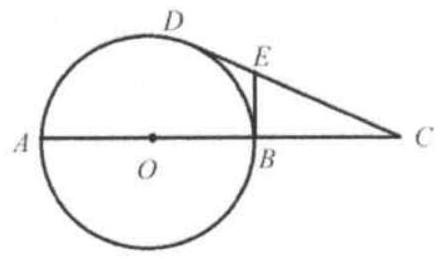
\includegraphics[width=\textwidth]{images/problem_image_1.jpg}

\section*{Solution}
Connect \(O B\).\\
Since both \(C D\) and \(B E\) are tangents of circle, \(B E=D E\).\\
Since \(D E=\frac{1}{2} E C, B E=\frac{1}{2} E C\). So \(\angle C=30^{\circ}\). Thus \(O C\) \(=2 O D\).\\
Since \(O B=O D, C B=O C-O B=O C-O D=2 O D-\)\\
\centering
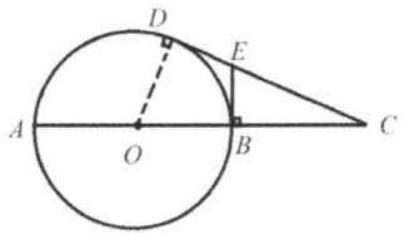
\includegraphics[width=\textwidth]{images/reasoning_image_1.jpg}\\
\(O D=O D=O B=O A\).\\
Thus \(C A=3 C B\).\\
We know that \(C D^{2}=C A \times C B=\frac{1}{3} C A^{2}\).\\
So \(C A^{2}=3 C D^{2} \quad \Rightarrow \quad C A=\sqrt{3} C D\).

\end{document}
